\documentclass[letterpaper]{article}

\usepackage{graphicx}
\usepackage{mathtools}
\usepackage{enumerate}
\usepackage[letterpaper,left=1.25in,right=1.25in,top=1in,bottom=1in]{geometry}
\usepackage{fancyhdr}
\usepackage[parfill]{parskip}
\usepackage{changepage}

\pagestyle{fancy}
\fancyfoot{}
% header/footer settings
\lhead{Kevin Nash (kjn33)}
\chead{EECS 391 -- P2}
\rhead{\today}
\cfoot{\thepage}

\begin{document}

\section{Linear Decision Boundaries}

\subsection{Plotting Iris Classes}
This project is written in Python, using Pandas dataframes to manipulate data
and Matplotlib to plot it.

The data is initialized like so,
\begin{verbatim}
# Read the file into a Pandas dataframe
iris_data = pd.read_csv(filename)
# Capitalize the column names and remove underscores
iris_data.columns = ["Sepal Length", "Sepal Width", "Petal Length",
                     "Petal Width", "Species"]
# Remove any species other than those specified by the assignment
iris_data = iris_data.loc[iris_data["Species"].isin(["versicolor", "virginica"])]
# Select the versicolor and virginica species individually
versi_data = iris_data.loc[iris_data["Species"] == "versicolor"]
virgi_data = iris_data.loc[iris_data["Species"] == "virginica"]
\end{verbatim}
The assignment asks us to consider only the versicolor and virginica species.
Let's take a look at the first few rows of each.
\begin{verbatim}
In [2]: versi_data.head(3)
    Sepal Length  Sepal Width  Petal Length  Petal Width     Species
50           7.0          3.2           4.7          1.4  versicolor
51           6.4          3.2           4.5          1.5  versicolor
52           6.9          3.1           4.9          1.5  versicolor

In [3]: virgi_data.head(3)
     Sepal Length  Sepal Width  Petal Length  Petal Width    Species
100           6.3          3.3           6.0          2.5  virginica
101           5.8          2.7           5.1          1.9  virginica
102           7.1          3.0           5.9          2.1  virginica
\end{verbatim}
We are interested in the petal dimensions. To plot them:
\begin{verbatim}
fig = plt.figure()
ax = fig.add_subplot(111)
ax.scatter(x=dataset_1["Petal Length"], y=dataset_1["Petal Width"],
           color="b", marker="o", label="versicolor")
ax.scatter(x=dataset_2["Petal Length"], y=dataset_2["Petal Width"],
           color="r", marker="^", label="virginica")
plt.xlabel("Petal Length (cm)")
plt.ylabel("Petal Width (cm)")
plt.legend(loc="upper left")
plt.savefig("plot_1a.pdf", bbox_inches="tight")
\end{verbatim}
This gives us
\begin{center}
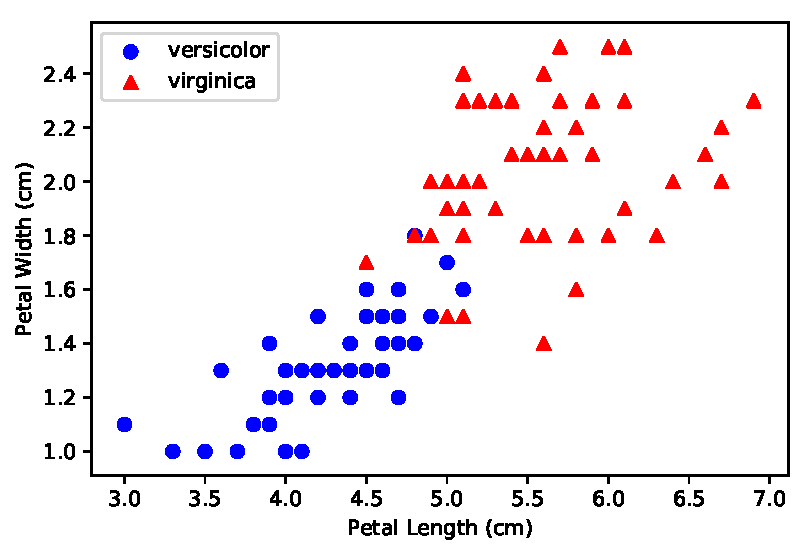
\includegraphics{plot_1a.pdf}
\end{center}
It is clear that at least two points of different classes overlap, which means
that our data is not going to be linearly separable.

\subsection{Choosing a Boundary by Hand}

I chose a boundary by physically drawing a line on the above plot using an
image editor. The line reaches from 2.4 on the y-axis to 6.5 on the x-axis.
Then we can get an equation in slope-intercept form from the coordinates
$(3, 2.4), (6.5, 1)$. $y=mx+b$ where $m=-0.4$ and $b=3.6$.

The code to generate this plot is identical to the above plot, except the line
\begin{verbatim}
plt.plot([3, 6.5], [2.4, 1], color="k", linestyle="-", linewidth=1)
\end{verbatim}
is now added before saving.
\begin{center}
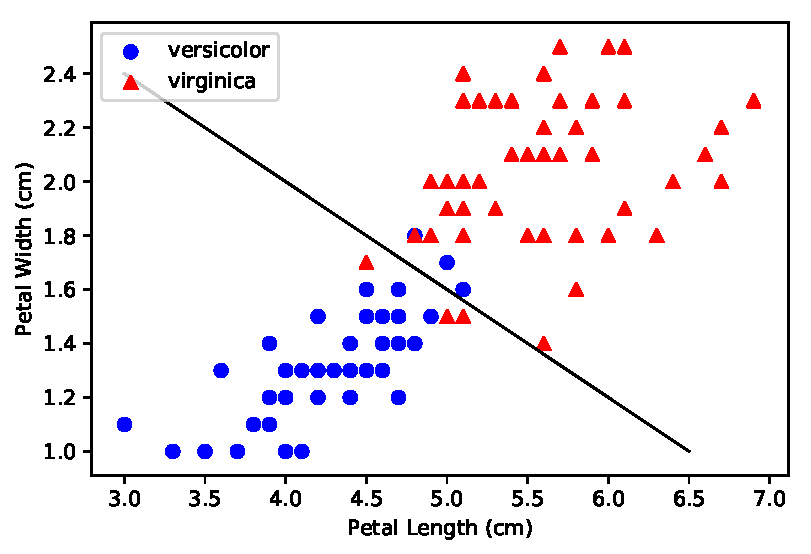
\includegraphics{plot_1b.pdf}
\end{center}

\subsection{Defining a Threshold Classifier}

We can now define a threshold classifier using the above parameters to compare
against our data points. Simply put, if the point is above the line, it is
predicted to be virginica. Otherwise it is predicted to be versicolor.

The calculation is shown here, where $x$ and $y$ correspond to $petal\ length$
and $petal\ width$, respectively.
\begin{verbatim}
""" Returns the distance from point (x,y) to the line in slope-intercept form """
def dist_from_line(x, y, m, b):
    return y - (m * x + b)

""" Returns "virginica" if the point (length, width) is above the line """
def classify_linear(row, slope, intercept):
    if 0 < dist_from_line(row["Petal Length"], row["Petal Width"], slope, intercept):
        return "virginica"
    return "versicolor"
\end{verbatim}

To plot this data, we isolate the misclassified points into their own dataframes.
Misclassified points are defined as those for which $Species \neq Classification$.
\begin{verbatim}
# Classify data linearly for part 1c
iris_data["Classification"] = iris_data.apply(
    lambda row: classify_linear(row, -0.4, 3.6), axis=1
)
misclassified = pd.DataFrame(columns=iris_data.columns)

for i, row in iris_data.iterrows():
    if not row["Classification"] == row["Species"]:
        misclassified.loc[len(misclassified.index)] = row

print("Linear decision accuracy: {}%".format(100 - len(misclassified.index) /
      len(iris_data.index) * 100))

versi_class = misclassified.loc[misclassified["Species"] == "versicolor"]
virgi_class = misclassified.loc[misclassified["Species"] == "virginica"]
plot_linear_bound(versi_class, virgi_class, "plot_1c.pdf")
\end{verbatim}
This threshold classifier misclassifies six data points, as shown in the next
plot. Note that points \textit{above} the line are supposed to be virginica
(red triangles), and points \textit{below} the line are supposed to be
versicolor (blue circles), but the opposite is true of misclassified points.
\begin{center}
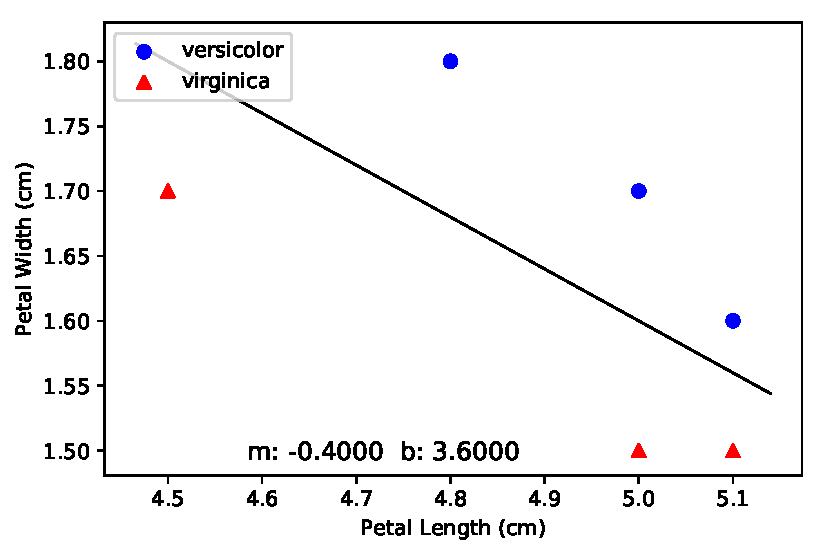
\includegraphics{plot_1c.pdf}
\end{center}

\subsection{Circle Decision Boundaries}

Instead of defining our decision boundary with a straight line, we can use
a circle instead. The technique is the same, although in this case the decision
is made considering whether a point is inside or outside of the circle, rather
than above or below a line. The functions are similar to those first shown in
section 1.3.
\begin{verbatim}
""" Returns the distance from point (x,y) to the edge of the circle """
def dist_from_circle(x, y, x_circ, y_circ, r):
    return ((x - x_circ)**2 + (y - y_circ)**2)**0.5 - r

""" Returns "virginica" if the point (length, width) is outside of the circle """
def classify_circular(row, x, y, radius):
    if 0 < dist_from_circle(row["Petal Length"], row["Petal Width"], x, y, radius):
        return "virginica"
    return "versicolor"
\end{verbatim}
Now we need to pick parameters for our circle ($x_{0}, y_{0}, r$). The
assignment instructs us to pick three sets. I started at the center of the plot
with an arbitrary radius of $\frac{1}{2}$. This, predictably, didn't give great
results, but with two adjustments the decision accuracy eventually met that of
the linear threshold ($94\%$). The parameters and results are shown below,
followed by the plot of each. Note that because the $x,y$ scales are not $1:1$,
the circle is \textit{mathematically} circular, \textit{not graphically} circular.
\begin{center}
\begin{tabular}{|c|c|c|c|}
\hline
$x$ & $y$ & $r$ & Accuracy\\
\hline
$4.75$ & $1.7$ & $0.5$ & 58\%\\
\hline
$4.5$ & $1.2$ & $0.5$ & 79\%\\
\hline
$4.0$ & $1.2$ & $1$ & 94\%\\
\hline
\end{tabular}
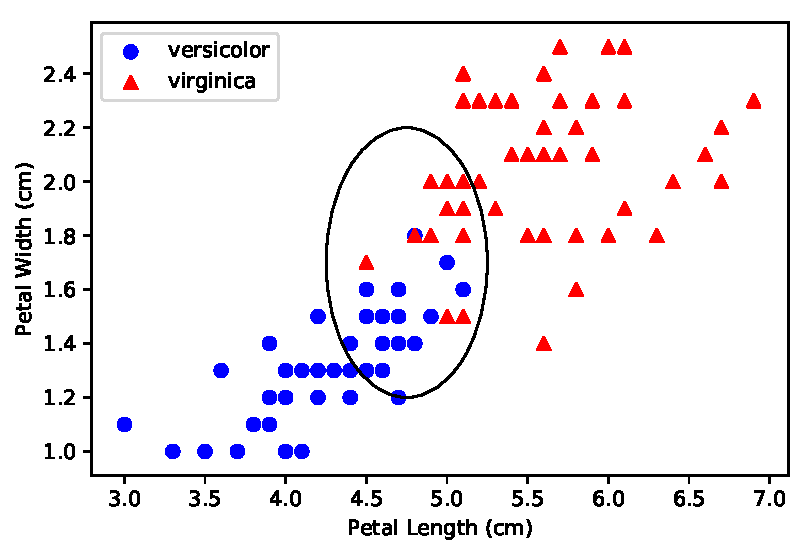
\includegraphics{plot_1d_1.pdf}
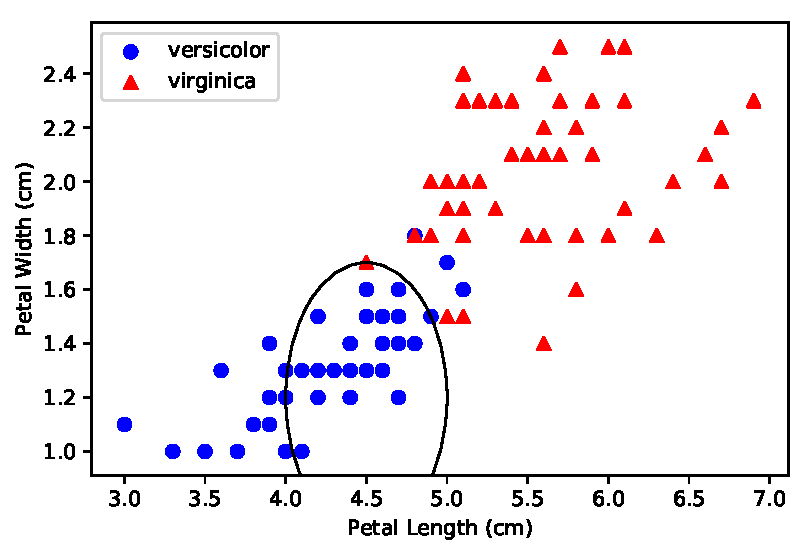
\includegraphics{plot_1d_2.pdf}
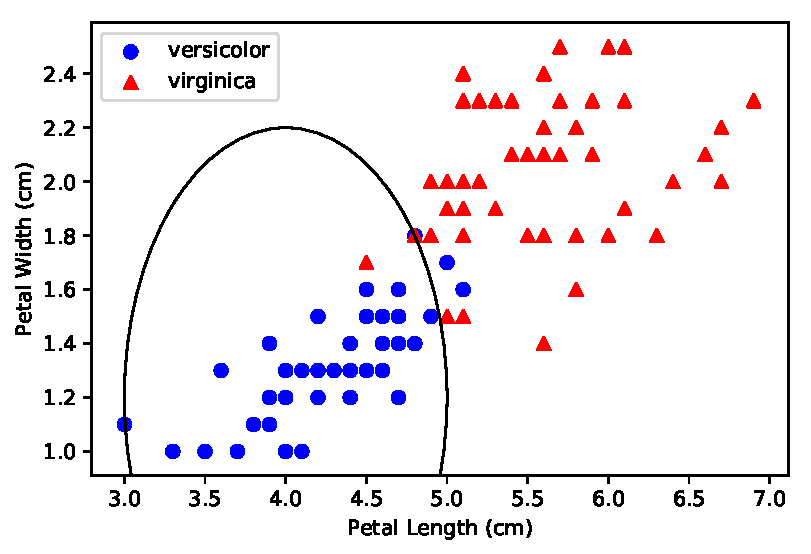
\includegraphics{plot_1d_3.pdf}
\end{center}

The plotting code is easy to imagine. Instead of drawing a line, just draw
a circle according to
\begin{verbatim}
circle = plt.Circle((x, y), r, color="k", fill=False)
ax.add_artist(circle)
\end{verbatim}

\section{Objective Functions}

\subsection{Calculating Mean-Squared Error}

The mean squared error is given by
\begin{equation*}
E = \frac{1}{2}\sum_{n=1}^N\left(\boldsymbol{w}^T\boldsymbol{x}_n-c_n\right)^2
\end{equation*}
In our case the predicted and actual values are $\boldsymbol{w}^T\boldsymbol{x}_n$
and $c_n$, where class of $x$ in pattern vector $\boldsymbol{x}_n$ is given by
\[
    x \in
    \begin{cases}
    \text{class 1} & \text{if } y\geq 0\\
    \text{class 2} & \text{if } y < 0
    \end{cases}
\]
and we can number the classes $0$ or $1$ to give $c_n$ a value according to
\[
    c_n =
    \begin{cases}
    0 & \boldsymbol{x}_n \in \text{class 1}\\
    1 & \boldsymbol{x}_n \in \text{class 2}
    \end{cases}
\]
However by this definition, $(\boldsymbol{x}_n-c_n)\subset \{-1,0,1\}$ and
therefore $(\boldsymbol{x}_n-c_n)^2\subset \{0,1\}$. The mean of zeroes and
ones doesn't give us a very percise error value, and so we can redefine the
first term. Rather than assigning a zero or a one based on the predicted class,
we can plug distance into a modified version of the sigmoid function, shown
below.
\begin{equation*}
x = \frac{1}{1+10^{-d}}
\end{equation*}
where $d$ is the distance from the decision boundary. By making this change,
we qualify our predictions with a degree of confidence.
 
\subsection{Examples of Large and Small Errors}
\subsection{Derivation of the Gradient}
\subsection{Gradients in Scalar and Vector Form}
\subsection{Summing the Gradient for an Ensemble of Patterns}

\section{Learning a Decision Boundary Through Optimization}

\subsection{Implementing Gradient Descent}
\subsection{Showing the Learning Curve}
\subsection{Illustration with Random Weights}
\subsection{Choosing the Gradient Step Size}
\subsection{Choosing the Stopping Criterion}

\end{document}